\documentclass[11pt]{article}
\usepackage[utf8]{inputenc}
\usepackage{polski}
\usepackage{graphicx}
\usepackage{array}
\usepackage{paralist}
\usepackage{verbatim}
\usepackage{subfig}
\usepackage{amsmath}
\usepackage{float}
\usepackage{amsthm}
\usepackage{amssymb}
\usepackage{pdfpages}
\usepackage{amsfonts}
\usepackage{tikz}
\usepackage{wasysym}
\usepackage[linguistics]{forest}
\usetikzlibrary{shapes,backgrounds}
\usepackage[margin=1in]{geometry}
\setlength\parindent{0pt}
\theoremstyle{definition}
\newtheorem{zadanie}{Zadanie}
\numberwithin{zadanie}{subsection}
\DeclareRobustCommand{\stirling}{\genfrac\{\}{0pt}{}}
\renewcommand*{\proofname}{Rozwiązanie}
\newtheorem{theorem}{Twierdzenie}
\title{Matematyka dyskretna}
\author{Igor Nowicki}
\begin{document}
\maketitle
\section{Ściągawka}

\subsection{Kategorie zadań}

\begin{figure}[H]
    \centering
    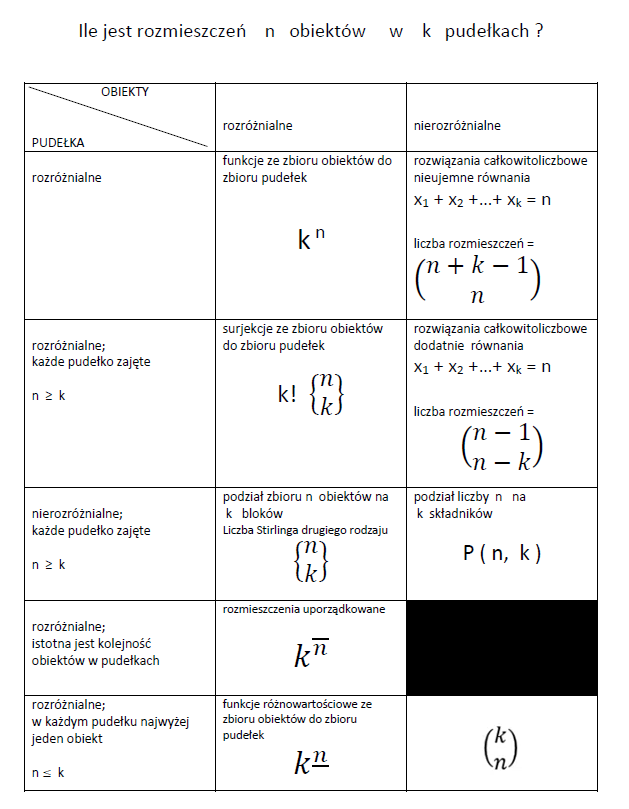
\includegraphics[width=0.7\linewidth]{cheatsheet.png}
\end{figure}

\subsection{Liczby Stirtlinga drugiego rodzaju i liczby Bella}

\textbf{Liczba Stirlinga drugiego rodzaju} $n\brace k$ odpowiada na pytanie na ile sposobów zbiór $n$ elementowy można podzielić na $k$ rozłącznych podzbiorów. \textbf{Liczba Bella} $B_n$ jest natomiast definiowana jako liczba wszystkich możliwych podziałów zbioru $n$-elementowego na podzbiory.

\begin{figure}[H]
    \centering
    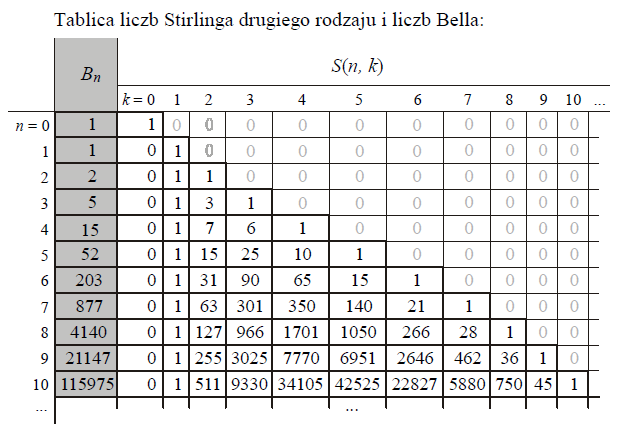
\includegraphics[width=0.7\linewidth]{bell2.png}
\end{figure}

\subsection{Liczba podziałów}

$P(n,k)$ - podział liczby $n$ na $k$ składników. Opisywane przez diagramy Ferrersa.

$P(n)$ - liczba niezerowych podziałów liczby $n$.

\begin{figure}[H]
    \centering
    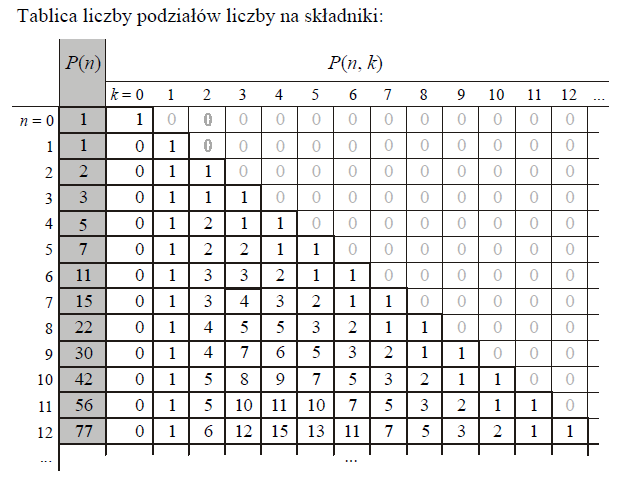
\includegraphics[width=0.7\linewidth]{podzial.png}
\end{figure}



\section{Zakres tematyczny}

\subsection{Zliczanie funkcji; zliczanie podzbiorów; zliczanie relacji}

\begin{zadanie}
    Dane są dwa zbiory:

    $$A = \{a,1,b,\{a,b\}\}, B = \{a,1,b,\{a,1\},2\}.$$

    \begin{enumerate}[a)]
        \item Ile jest wszystkich funkcji $f: A \to B$?
        \item Ile jest funkcji różnowartościowych $g: B \to A$?
        \item Ile jest funkcji różnowartościowych $g: B \to P(A)$?
        \item Ile jest wszystkich relacji w zbiorze B?
        \item Ile jest wszystkich surjekcji $h: B \to A$?
        \item Ile jest wszystkich surjekcji $s: A \to B$?
        \item Ile jest wszystkich bijekcji $b: B\to B$?
        \item Ile podzbiorów ma zbiór $P (A\times B)$? \{definicja: P (Y) = zbiór wszystkich podzbiorów zbioru Y\}
        \item Jaką część wszystkich relacji, dających się określić w zbiorze B, stanowią relacje równoważności?
        \item Ile relacji równoważności można zdefiniować w zbiorze B?
    \end{enumerate}
\end{zadanie}
\begin{proof}
    \begin{itemize}
        \item Moc zbioru $|A| = 4$,
        \item moc zbioru $|B| = 5$,
        \item moc zbioru $|P(A)| = 2^4 = 16$,
        \item moc zbioru $|P(B)| = 2^5=32$.
    \end{itemize}
    \begin{enumerate}[a)]
        \item Ile jest wszystkich funkcji $f: A \to B$?

              Odwzorować z $A$ do $B$ jest $5^4$. Bierze się to z faktu, że każdemu z $4$ elementów $A$ (obiektów) możemy przypisać dokładnie jeden z $5$ elementów $B$ (pudełek). Korzystamy ze wzoru na $n$ rozróżnialnych obiektów w $k$ rozróżnialnych pudełkach: $k^n = 5^4$.

        \item Ile jest funkcji różnowartościowych $g: B \to A$?

              Nie ma żadnych funkcji różnowartościowych - przynajmniej element zbioru $A$ będzie wskazywany przez dwa elementy zbioru $B$ (zasada Dirichleta).

        \item Ile jest funkcji różnowartościowych $g: A \to B$?

              Bierzemy pierwszy element $A$, możemy mu przypisać jeden z 5 elementów $B$. Kolejnemu możemy przypisać już tylko jeden z 4 elementów, potem jeden z 3... i tak dalej, 4 razy. Odpowiedź to $5^{\underbar{4}} = 5\cdot4\cdot3\cdot2$.

        \item Ile jest funkcji różnowartościowych $g: B \to P(A)$?

              Analogiczna odpowiedź: z $n=5$ do $k=2^4=16$. W każdym pudełku co najwyżej jeden obiekt, $k^{\underbar n} = 16^{\underbar 5}$.

        \item Ile jest wszystkich surjekcji $h: B \to A$?

              Odpowiedź jest ta sama jak na pytanie "na ile sposobów 5 rozróżnialnych elementów możemy umieścić w 4 pudełkach tak, aby w każdym pudełku był przynajmniej 1 element"? Odpowiedzią na to pytanie jest $k!{n\brace k}$, gdzie $k$ jest liczbą pudełek (4), a $n$ - liczbą obiektów (5). W tym wypadku mamy $4!{5\brace 4} = 4!\cdot10 = 240$ kombinacji.

        \item Ile jest wszystkich surjekcji $s: A \to B$?

              Oczywiście niemożliwe jest rozłożyć 4 elementy do 5 pudełek tak, by każde pudełko miało przynajmniej jeden element. Odpowiedź to zero.

        \item Ile jest wszystkich bijekcji $b: B\to B$?

              Odpowiadamy na pytanie, ile jest permutacji zbioru $5$-elementowego. Odpowiedzią jest oczywiście $5! = 120$.

        \item Ile podzbiorów ma zbiór $P (A\times B)$? \{definicja: P (Y) = zbiór wszystkich podzbiorów zbioru Y\}

              Liczba podzbiorów zbioru $X$ jest równa mocy zbioru potęgowego, $|P(X)| = 2^{|X|}$. W tym wypadku bierzemy zbiór będący iloczynem kartezjańskim, o mocy 20 elementów - odpowiedzią jest $2^{20} = 1024\cdot1024\approx 1,000,000$.


        \item Ile jest wszystkich relacji równoważności w zbiorze B?

              Relacja równoważności jest określana jednoznacznie przez podział elementów na klasy abstrakcji - takie klasy są zawsze rozłączne. Pytamy zatem, na ile sposobów możemy rozdzielić zbiór $5$ elementów na rozłącznie podzbiory.

              Odpowiedź na pytanie "ile jest podziałów zbioru $n$-elementowego na $k$ bloków" daje \textbf{liczba Stirlinga drugiego rodzaju}, $n\brace m$. Natomiast suma wszystkich możliwych podziałów, tj. $B_n = \sum_{k=1}^n {n\brace k}$, jest dana jako \textbf{liczba Bella}.

              Rozwiązaniem jest $B_5 = 52$.

        \item Jaką część wszystkich relacji, dających się określić w zbiorze B, stanowią relacje równoważności?

              Wszystkie relacje w zbiorze $B$ jest równa wszystkim możliwym macierzom binarnym $|B|\times|B|$, tj. $2^{25}$ macierzom. Liczba wszystkich relacji równoważności odpowiada liczbie Bella $B_{5}$, co jest równe 52.

    \end{enumerate}

\end{proof}

\begin{zadanie}
    X - zbiór 5-elementowy, Y - zbiór 4-elementowy, Z - zbiór 9-elementowy

    a = liczba takich relacji równoważności w  zbiorze Z które mają co najmniej siedem klas abstrakcji.

    b = liczba surjekcji $X\to Y$.

    Która liczba jest większa: a czy b? Uzasadnij.
\end{zadanie}
\begin{proof}
    Skorzystamy z tabeli liczb Stirlinga.

    Liczba wszystkich podziałów zbioru $n$-elementowego na $k$ części to liczba Stirlinga drugiego rodzaju:

    $$\stirling nk.$$

    Potrzebujemy liczbę wszystkich podziałów na 7, 8 lub 9 bloków - odpowiadają im liczby Stirlinga $\stirling97,\stirling98,\stirling99$. Z tabeli wyczytujemy, że odpowiadają im, kolejno: $462, 36, 1$. Ich suma wynosi $499$.

    $a = \stirling97 + \stirling98 + \stirling99 = 462, 36, 1 = 499.$

    Zliczanie surjekcji $X\to Y$ oznacza policzenie wszystkich sposobów tworzenia czterech niepustych zbiorów ze zbioru 5 elementów, razy liczba kombinacji 4 elementów.

    $$b = \stirling54\cdot4!.$$

\end{proof}

\subsection{Zbiory z powtórzeniami; funkcje tworzące; zastosowanie funkcji tworzących do zliczania rozwiązań nierówności}

\begin{zadanie}
    \begin{enumerate}
        \item Zbadaj, ile rozwiązań ma nierówność: $x_1 + x_2 + x_3 \leq 8$, gdzie $x_1, x_2, x_3$ są
              liczbami całkowitymi nieujemnymi, a dodatkowo spełnione są warunki: $x_1$ - parzysta,
              $x_2 = 0$ lub $1, 2 < x_3 < 5$.
        \item Ile rozwiązań ma podwójna nierówność:$ 5 < x_1 + x_2 + x_3 \leq 8$, przy czym warunki
              na zmienne są takie same jak w podpunkcie 1 ?
        \item Zbadaj, ile rozwiązań ma nierówność: $x_1 + x_2 + x_3 \leq 8$,
              gdzie $x_1 , x_2 , x_3 $są liczbami całkowitymi nieujemnymi, a dodatkowo spełnione są warunki:
              $x_1$ - parzysta, $x_2 = 0 lub 1$, $x_3$ podzielne przez $3$.
    \end{enumerate}
\end{zadanie}
\begin{proof}

    \begin{enumerate}[a)]
        \item Musimy policzyć sumę przypadków:
              \begin{itemize}
                  \item $x_1$ parzysta, $x_2 = 0$,
                  \item $x_1$ parzysta, $x_2$ dowolna, $x_3 \in \{3,4\}$,
                  \item $x_1$ parzysta, $x_2 = 0$ oraz $x_3 \in \{3,4\}$.
              \end{itemize}

              Pierwszy przypadek możemy policzyć poprzez wygenerowanie funkcji tworzącej $f(x)=(1+x^2+x^4+x^6+x^8)\cdot(1+x+x^2+x^3+x^4+x^5+x^6+x^7+x^8)$ i policzenie sumy wszystkich argumentów dla potęg mniejszych lub równych od 8 dla wymnożonych wielomianów - wynik to 25.

              Drugi przypadek atakujemy w ten sam sposób, z tym że mamy funkcję tworzącą $f(x)= (1+x^2+x^4+x^6+x^8)\cdot(1+x+x^2+x^3+x^4+x^5+x^6+x^7+x^8)\cdot(x^3+x^4) = O(x^9) + 6 x^8 + 5 x^7 + 4 x^6 + 3 x^5 + 2 x^4 + x^3$, co daje 21 rozwiązań.

              Trzeci przypadek daje nam $f(x)= (1+x^2+x^4+x^6+x^8)\cdot1\cdot(x^3+x^4) = x^3+x^4+x^5+x^6+x^7+x^8+O(x^9)$, co daje sumę 6 rozwiązań.

              Aby policzyć wszystkie rozwiązania, skorzystamy z zasady włączania/wyłączania, tj. $|A\cup B| = |A|+|B| - |A\cap B| = 25+21-6 = 40$ rozwiązań.
    \end{enumerate}
\end{proof}


\begin{zadanie}

    $X = <5a,4b,3c>$; rozważ takie podzbiory, w których a występuje parzystą liczbę razy,
    b występuje najwyżej dwa razy, ale co najmniej raz, c występuje co najmniej dwa razy.
    Skonstruuj funkcję tworzącą dla ciągu liczb podzbiorów k-elementowych, przy zadanych
    warunkach dla $a, b, c.$
    \begin{enumerate}
        \item Ile takich podzbiorów zawiera więcej niż 6 elementów?
        \item Ile takich podzbiorów zawiera 4 elementy lub 8 elementów?
    \end{enumerate}
\end{zadanie}
\begin{proof}
    Warunki zamieniają się w następujący wielomian dla funkcji tworzącej:

    $$f(x) = (1+x^2+x^4)\cdot(1+x+x^2)\cdot(x^2+x^3) = x^9 + 2 x^8 + 3 x^7 + 3 x^6 + 3 x^5 + 3 x^4 + 2 x^3 + x^2$$

    \begin{enumerate}
        \item Ile takich podzbiorów zawiera więcej niż 6 elementów?

              Pytamy o współczynniki przy potęgach wyższych niż 6: $1+2+3 = 6$.

        \item Ile takich podzbiorów zawiera 4 elementy lub 8 elementów?

              Pytamy o sumę współczynników przy potęgach 4 oraz 8: $3+2 = 5$
    \end{enumerate}
\end{proof}

\subsection{Podział zbioru na bloki - liczby Stirlinga II rodzaju; liczby Bella - zliczanie relacji równoważności; zliczanie surjekcji}

\begin{zadanie}
    Z osób $\{a,b,c,d,e,f,g,h\}$ tworzymy 4 niepuste zespoły.

    \begin{enumerate}[a)]
        \item Ile jest sposobów stworzenia zespołów?
        \item Ile jest sposobów przy warunkach: $a,b$ muszą być w jednym zespole oraz ani $c$, ani $d$ nie mogą być razem z $a$ oraz $b$.
    \end{enumerate}
\end{zadanie}
\begin{proof}
    Korzystamy z modelu podziału na bloki.
    \begin{enumerate}[a)]
        \item Dla braku warunków rozwiązaniem będzie prosty podział na bloki: $P(n,k) = P(8,4) = \stirling 84$.
        \item Przy narzuconym warunku traktujemy zbiór jako 7-elementowy (a oraz b muszą być zawsze razem). Od takiego zbioru odejmujemy liczbę przypadków w których $c$ jest razem z $(a,b)$, $d$ jest razem z $(a,b)$ oraz $c$ i $d$ są razem z $(a,b)$.

              \begin{itemize}
                  \item Liczba przypadków $c$ razem z $(a,b)$: $\stirling64$,
                  \item Liczba przypadków $d$ razem z $(a,b)$: $\stirling64$,
                  \item Liczba przypadków $c,d$ razem z $(a,b)$: $\stirling54$,
              \end{itemize}

              Suma wszystkich przypadków $(a,b)$ bez $c$ lub $d$: $X= \stirling64+\stirling64-\stirling54 = 120$.

              Całkowita liczba przypadków: $\stirling74 - ( 2\stirling64 - \stirling54 ) = 230.$
    \end{enumerate}
\end{proof}

\begin{zadanie}
    $X=\{a,b,c,d,e\}$. $Y=\{1,2,3\}$. Ile jest funkcji $g: X\to Y$ takich, że $|g^{-1}(\{3\})| = 2$?
\end{zadanie}
\begin{proof}
    Pytamy o liczbę przypadków, w których w pudełku $3$ są dokładnie dwa elementy z $X$. Możemy wybrać dwa elementy ze zbioru $5$ elementowego na $\binom52$ sposobów. Następnie, chcemy przyporządkować pozostałe trzy elementy do dowolnych dwóch pozostałych pudełek: $2^3$ możliwości. Razem mamy $\binom52\cdot2^3 = 80$ kombinacji.
\end{proof}

\subsection{Podziały liczby na składniki}

\begin{zadanie}
    18 pięciozłotowych monet wrzuciliśmy do czterech identycznych puszek. Oblicz liczbę kombinacji, jeśli:
    \begin{enumerate}[a)]
        \item W każdej puszce są co najmniej 3 monety.
        \item W każdej puszce musi się znaleźć parzysta i niezerowa suma.
    \end{enumerate}
    Diagramy Ferrisa.
\end{zadanie}
\begin{proof}
    Przy braku warunków mielibyśmy przypadek podziału 18 na 4 lub 3 lub 2 lub 1 skadników, czyli $P(18,4)+P(18,3)+P(18,2)+P(18,1)$, lub po prostu $p(18)$, gdzie $p$ jest zliczaniem wszystkich możliwych podziałów.

    Dla przypadków opisanych w warunkach:

    \begin{enumerate}[a)]
        \item W każdej puszce są co najmniej 3 monety.

              Skorzystamy z tego założenia by uprościć sobie rozwiązywanie. Jeśli wrzucimy do każdej puszki po dwie monety, to pozostaje nam 10 monet do rozdysponowania na 4 niezerowe składniki - zatem $P(10,4)$.

        \item W każdej puszce musi się znaleźć parzysta i niezerowa suma.

              Możemy potraktować układ jako równoważny z wrzucaniem 9-ciu par monet do puszek. W ten sposób lądujemy z $P(9,4)=6$ przypadkami.
    \end{enumerate}

\end{proof}

\begin{zadanie}
    Do trzech jednakowych puszek wrzucono 9 monet groszowych: 1, 2, 5, 10, 20, 50 oraz złotowych: 1, 2, 5.

    Ile jest sposobów wrzucenia jeśli:
    \begin{enumerate}
        \item w każdej puszcze znalazła się jakaś moneta

        \item nie ma ograniczeń jak w wersji 1
    \end{enumerate}

\end{zadanie}
\begin{proof}
    Zadanie polega na rozmieszczeniu \textbf{rozróżnialnych} elementów na nierozróżnialne zbiory - jest ono równoważne z pytaniem o liczbę podziałów na trzy klasy abstrakcji (w przypadku 1) lub po prostu o liczbę podziałów na klasy abstrakcji (w przypadku 2).

    Dla przypadku pierwszego mamy liczbę podziałów w postaci liczby Stirlinga $\stirling 9 3=3025$. W drugim przypadku mamy odpowiedź w postaci sumy podziałów na trzy, dwa lub jedno pudełko: $\stirling93+\stirling92+\stirling91=3281$.
\end{proof}

\begin{zadanie}
    Ile jest podziałów liczby 20 na 8 składników?
\end{zadanie}
\begin{proof}
    Oczywiście odpowiedzią będzie $P(20,8)$. Spróbujemy uzyskać tę liczbę z mniejszych sum, na podstawie wzoru:

    $$P(n,k) = \sum_{i=0}^kP(n-k,i),$$

    czyli w tym wypadku będzie to:

    $$P(20,8) = P(12,0)+P(12,1)+\ddots+P(12,8)=70.$$
\end{proof}
\begin{zadanie}
    Ile jest podziałów liczby 13 na 4 składniki, w których największy składnik jest nie mniejszy niż 4?
\end{zadanie}
\begin{proof}
    Oczywiście dzieląc 13 na 4 składniki musimy mieć największy składnik większy lub równy 4 - ze względu na zasadę szufladkową. Zatem $P(13,4)=18$.
\end{proof}

\begin{zadanie}
    20 jednakowych klocków włożono do 5 jednakowych pudełek. Pudełka są niepuste. W jednym z pudełek są dokładnie 4 klocki. Ile jest takich sposobów rozłożenia klocków?
\end{zadanie}
\begin{proof}
    Oczywiście musimy wykluczyć jedno pudełko z czterema klockami, co redukuje nasz układ do 16 jednakowych klocków w 4 jednakowych pudełkach. Sposobów rozmieszczenia jest oczywiście $P(16,4)=P(12,1)+P(12,2)+P(12,3)+P(12,4)=34$.
\end{proof}

\begin{zadanie}
    Dane jest 10 jednakowych zadań na 4 jednakowe maszyny. Każda z maszyn musi pracować (mieć przynajmniej jedno zadanie). Ile jest sposobów przydziału zadań do maszyn?
\end{zadanie}
\begin{proof}
    Odpowiedź to $P(10,4)$.
\end{proof}

\begin{zadanie}
    Dane jest 8 rozróżnialnych zadań na 4 jednakowe maszyny. Każda z maszyn pracuje. Na jednej z maszyn są dokładnie 2 zadania. Ile jest sposobów?
\end{zadanie}
\begin{proof}
    Po pierwsze, wybieramy 2 zadania na $\binom 82$ sposobów. Po drugie, mnożymy wynik przez $\stirling63$. Wynik to:

    $$\binom82\cdot \stirling63 = 2520.$$
\end{proof}
\begin{zadanie}
    Mamy 8 rozróżnialnych zadań dla 4 rozróżnialnych maszyn. Każda z maszyn pracuje.
\end{zadanie}
\begin{proof}
    Wynik to $4!\cdot\stirling 84 = 40824$.
\end{proof}
\begin{zadanie}
    12 identycznych piłek wkładamy do jednakowych toreb. W torbie mieszczą się najwyżej 4 piłki. Na ile sposobów możemy to zrobić? Wyjaśnij.
\end{zadanie}
\begin{proof}
    Przypadek podziału 12 identycznych elementów do toreb gdzie najwięcej możemy upakować 4 elementy na raz jest identyczny z przypadkiem podziału na 4, 3, 2 oraz 1 zbiór. Odpowiedź to:

    $$P(12,4)+P(12,3)+P(12,2)+P(12,1)=34.$$
\end{proof}

\begin{zadanie}
    Zdajemy test z analizy. Jest 5 zadań z granic funkcji, 2 zadania z ekstremów, 3 zadania z całek, 2 zadania z równań różniczkowych. Każde zadanie jest za 1 punkt. Test jest zaliczony, gdy uzyskamy co najmniej 4 punkty. Warunki: musimy rozwiązać nie więcej niż 2 zadania z granic, przynajmniej jedno zadanie z całek i przynajmniej jedno zadanie z równań różniczkowych.

    Ile jest różnych zestawów zaliczających?
\end{zadanie}
\begin{proof}
    Zadanie możemy przedstawić w sposób formalny. Zliczamy liczbę podzbiorów przynajmniej czteroelementowych zbioru z powtórzeniami:

    $$<5g,2e,3c,2r>,$$

    dla którego podzbiory muszą mieć najwyżej $2g$, przynajmniej $1c$ oraz przynajmniej $1r$.

    Zadanie można przetłumaczyć na formę $<2g,2e,3c,2r>,$ ponieważ możemy rozwiązać maksymalnie 2 zadania z granic.

    Najprościej jest zastosować tutaj metodę funkcji tworzących:

    $$f(x) = (1+x+x^2)\cdot(1+x+x^2)\cdot(x+x^2+x^3)\cdot(x+x^2)=x^9+4x^8+9x^7+13x^6+13x^5+9x^4+4x^3+x^2.$$

    Bierzemy tylko potęgi równe lub większe od 4. Suma współczynników to $1+4+9+13+13+9=49$.

\end{proof}

\begin{zadanie}
10 rozróżnialnych zadań przypisujemy dowolnie do trzech identycznych maszyn. Na ile sposobów możemy to zrobić?
\end{zadanie}

\begin{proof}
Odpowiedź to suma podziałów na trzy maszyny (niepuste), dwie maszyny oraz jedną maszynę. Ponieważ są one nierozróżnialne, nie gra roli które wybierzemy. Odpowiedź to:

$$\stirling{10}{3}+\stirling{10}{2}+\stirling{10}{1}=9842.$$
\end{proof}

\subsection{Dobór modelu matematycznego do zadania zliczania}

\begin{zadanie}

    $$X=\{a,b,c,d,e,f\}.$$

    \begin{enumerate}[a)]
        \item Ile jest relacji równoważności w X które mają dwie klasy abstrakcji?
        \item Ile jest relacji równoważności w X takich, że ich klasy abstrakcji są mocy parzystej?

        \item Ile jest relacji równoważności w X takich, że ich klasy abstrakcji są mocy nieparzystej?

        \item Ile jest relacji równoważności w X, które mają dwie klasy abstrakcji?
    \end{enumerate}
\end{zadanie}
\begin{proof}
    \begin{enumerate}[a)]
        \item Szukamy podziału zbioru 6 elementowego na 2 niezerowe i nierozróżnialne bloki. Odpowiedź to liczba Stirlinga $\stirling 62$.
        \item
    \end{enumerate}
\end{proof}


% \begin{zadanie}
%     $$X = \{a,b,c,d,e,f\}$$

%     \begin{enumerate}
%         \item skonstruuj w X relację równoważności, która ma klasy abstrakcji $\{a,d,f\}, \{c,e\}, \{b\}$. Narysuj graf tej relacji.

%         \item Ile jest w X relacji równoważności, których klasy abstrakcji mają taką samą liczność jak klasy z podpunktu 1)?
%     \end{enumerate}

% \end{zadanie}
% \begin{proof}
%     \begin{enumerate}
%         \item a
%         \item b

%               $$\binom 63\binom 32\binom11$$
%     \end{enumerate}
% \end{proof}

% \begin{zadanie}
%     Na ile sposobów można przydzielić $n$ zadań do $m$ maszyn, jeśli:

%     \begin{itemize}
%         \item maszyny są rozróżnialne, zadania są rozróżnialne: $$$$
%     \end{itemize}
% \end{zadanie}

% \begin{zadanie}
%     Na ile sposobów sześć zadań ($z_1,z_2,z_3,z_4,z_5,z_6$) można przyporządkować do trzech maszyn ($m_1,m_2,m_3$).
% \end{zadanie}

% \begin{zadanie}
%     10 nierozróżnialnych zadań, 5 rozróżnialnych maszyn. Na ile sposobów?

%     Co jeśli m5 musi mieć 3 zadania?
% \end{zadanie}
% \begin{proof}
%     Szukamy rozwiązania równania:

%     $$m_1+m_2+m_3+m_4+m_5=10,$$

%     gdzie zakładamy, że maszyna może też być bezczynna (0 zadań).
% \end{proof}

% \begin{zadanie}
%     6 rozróżnialnych zadań, trzy jednakowe maszyny, nieistotna kolejność zadań. Żadna z maszyn nie może wykonywać więcej niż 3 zadania.

%     Na ile sposobów można przydzielić zadania do maszyn?
% \end{zadanie}
% \begin{proof}
%     Zadania grupujemy na trzy pakiety. Każde zadanie jest wykonywane.

%     Wykluczamy przypadki w których mamy podział 4,1,1. Takich przypadków jest $\binom62$. Przypadków podziału 6 zadań na trzy maszyny to $\stirling63$.

% \end{proof}
% \begin{zadanie}
%     8 rozróżnialnych zadań, 4 jednakowe maszyny, wszystkie pracują, na jednej z maszyn są dokładnie 2 zadania.
% \end{zadanie}
% \begin{proof}
%     Najpierw wybieramy dwa zadania spośród 8 bez uwzględnienia kolejności, co daje $\binom82$ możliwości. Następnie musimy rozdzielić 6 rozróżnialnych zadań na 3 zbiory, co daje $\stirling63=90$ możliwości.
% \end{proof}

% \begin{zadanie}
%     Zadania z1,z2,z3,z4,z5,z6, każde zadanie wykonane, maszyny m1,m2,m3,m4, każda pracuje.

%     Ile jest sposobów przydziału zadań.
% \end{zadanie}
% \begin{proof}
%     $$\stirling 84\cdot4!$$
% \end{proof}


% \begin{zadanie}
%     Mamy 6 rozróżnialnych zadań, dwie rozróżnialne maszyny.
% \end{zadanie}

% \begin{zadanie}
%     Przydzielamy 10 zadań rozróżnialnych do 3 maszyn rozróżnialnych. Warunki: m1 wykonuje dokładnie trzy zadania, m2 wykonuje co najmniej 4 zadania, wszystkie zadania rozdzielono. Ile jest takich przydziałów? Uzadsadnij.

%     \begin{itemize}
%         \item Każda maszyna pracuje.
%         \item Nie każda maszyna pracuje.
%     \end{itemize}
% \end{zadanie}
% \begin{proof}
%     \begin{itemize}
%         \item Każda maszyna pracuje: $$\binom {10}3*\Big(\binom73+\binom75+\binom76\Big)$$
%     \end{itemize}
% \end{proof}


% \begin{zadanie}
%     Przydzielamy 10 rozróżnialnych zadań do 4 rozróżnialnych maszyn. m1 wykonuje dokładnie 3 zadania, m2 wykonuje co najmniej 3 zadania, wszystkie zadania rozdzielono. Ile jest takich przydziałów?

%     \begin{itemize}
%         \item Każda maszyna pracuje.
%         \item Niekoniecznie każda maszyna pracuje.
%     \end{itemize}
% \end{zadanie}
% \begin{proof}


%     \begin{itemize}
%         \item Każda maszyna pracuje:

%               $$\binom{10}3 \cdot\Big(\binom73\cdot2!\stirling42+\binom74\cdot2!\stirling32+\binom75\cdot2!\stirling22\Big)$$

%     \end{itemize}
% \end{proof}


% \section{MDA Zadania powtórkowe cz. 2}

% % \begin{zadanie}
% %     Ile nieujemnych, całkowitoliczbowych rozwiązań ma równanie $x_1 + x_2 + x_3 + x_4 + x_5 = 20$,
% %     gdzie dodatkowo spełnione są warunki: $x_1 \geq 3, x_2 > 0, x_3 > 2, x_4 \geq 3, x_5 = 2$ ?
% %     (Wskazówka: dokonać podstawienia zmiennych)
% % \end{zadanie}
% % \begin{proof}
% %     Chcemy sprowadzić problem do przypadku kiedy poszukujemy rozwiązań dla wszystkich zmiennych $y_i\geq0$. Zastosujemy podstawienia:
% %     \begin{itemize}
% %         \item $y_1 = x_1 - 3$,
% %         \item $y_2 = x_2 - 1$,
% %         \item $y_3 = x_3 - 3$,
% %         \item $y_4 = x_4 - 3$,
% %     \end{itemize}
% %     natomiast za $x_5$ podstawimy wartość $2$. Dostajemy:

% %     $$(y_1 + 3) +(y_2+1) + (y_3+3) + (y_4+3) + 2=20,$$

% %     (podstawiając za $x_i$ nasze wartości). Po skróceniu:

% %     $$y_1 +y_2+1 + y_3+ + y_4=8,$$

% %     Co daje nam wynik $\binom{11}{3} = 165$.
% % \end{proof}

% % \begin{zadanie}
% %     W sklepie w koszu jest 40 jednakowych skarpet.

% %     8 (rozróżnialnych) klientów $\{a, b, c, d, e, f, g, h \}$ wybiera je z kosza.

% %     Na ile sposobów mogli to zrobić, jeśli: każdy klient coś kupił, każdy kupił parzystą liczbę skarpet i wszystkie skarpety
% %     zostały sprzedane?
% % \end{zadanie}
% % \begin{proof}
% % \end{proof}



% % \begin{zadanie}
% %     Siedem cukierków $\{ a, b, 1, 2, 3, 4, 5 \} $ wkładamy do 3 identycznych pudełek. W każdym
% %     pudełku musi być jakiś cukierek. Muszą być spełnione oba poniższe warunki:
% %     \begin{enumerate}
% %         \item a i b nie mogą się znaleźć razem w jednym pudełku;
% %         \item ani a, ani b nie mogą być same w pudełku.
% %     \end{enumerate}
% %     Ile jest takich podziałów?
% % \end{zadanie}
% % \begin{proof}
% % \end{proof}

% % \begin{zadanie}
% %     Osiem osób $\{a, b, c, 1, 2, 3, 4, 5\}$ ma usiąść przy 4 identycznych stolikach. Przy każdym
% %     stoliku ktoś musi usiąść. Warunek: żadna z par a,b; b,c; a,c; nie może siedzieć razem.
% %     Ile jest sposobów rozsadzenia tych osób?
% % \end{zadanie}
% % \begin{proof}
% % \end{proof}

% % \begin{zadanie}
% %     Mamy 9 obiektów ${ o1, \dots., o9 }$ i cztery pudełka ${ p1, p2, p3, p4 }$. Warunki: w pudełku
% %     p1 muszą się znaleźć dokładnie 3 obiekty oraz w każdym pudełku musi być przynajmniej
% %     jeden obiekt. Ile jest sposobów rozłożenia obiektów do pudełek?

% % \end{zadanie}
% % \begin{proof}
% % \end{proof}
% % \begin{zadanie}
% %     X - zbiór 5-elementowy; Y - zbiór 4-elementowy; Z - zbiór 9-elementowy.
% %     a = liczba takich relacji równoważności w zbiorze Z, które mają co najmniej siedem klas
% %     abstrakcji;
% %     b = liczba surjekcji $X \to Y$.
% %     Która liczba jest większa: a czy b? Uzasadnij.
% % \end{zadanie}
% % \begin{proof}
% % \end{proof}


% Podział liczby na składniki P(n,k).

% Diagram Ferrersa. Przedstawien

% \begin{zadanie}
%     Ile jest podziałów liczby 20 na 8 składników?

%     Odp.: 70
% \end{zadanie}
% \begin{proof}
%     Korzystając z tablicy podziałów na składniki, szukamy $P(20,8) = \sum_{i=0}^8P(20-8,i)$.
% \end{proof}

% \begin{zadanie}
%     Ile jest podziałów liczby 13 na 4 składniki, w których największy składnik jest niemniejszy niż 4? Uzasadnij.

%     Odp.: 18
% \end{zadanie}
% \begin{proof}
% \end{proof}

% \begin{zadanie}
%     $X = { a, b, c, d, e, f }$
%     \begin{enumerate}
%         \item Skonstruuj w X relację równoważności, która ma klasy abstrakcji:
%               { a, d, f }, { c, e }, { b }. Narysuj graf tej relacji.
%         \item Ile jest w X relacji równoważności, których klasy abstrakcji mają taką samą liczność jak
%               klasy z podpunktu 1)?
%     \end{enumerate}
%     Odp.: 60
% \end{zadanie}
% \begin{proof}
% \end{proof}

% \begin{zadanie}
%     $X = { a, b, c, 1, 2, 3, 4, 5, 6, 7}. $

%     Dzielimy zbiór X na cztery bloki, tak by w jednym z bloków
%     były a i b, ale nie było w nim c. Ile jest takich podziałów? Odp.: 6069

% \end{zadanie}
% \begin{proof}
% \end{proof}

% \begin{zadanie}
%     20 jednakowych klocków włożono do 5 jednakowych pudełek. Pudełka są niepuste. W
%     jednym z pudełek są dokładnie 4 klocki. Ile jest takich sposobów rozłożenia klocków?

%     Odp.: 34
% \end{zadanie}
% \begin{proof}
% \end{proof}

% \begin{zadanie}
%     10 rybek ${r1, r2, r3,\dots, r10}$ wpuszczamy dowolnie do trzech identycznych akwariów.
%     \begin{enumerate}
%         \item Ile jest wszystkich sposobów wpuszczenia rybek do akwariów? Odp.: 9842
%         \item Ile jest sposobów wpuszczenia rybek, jeśli r1, r2, r3, r4 muszą być razem w jednym
%               akwarium?
%     \end{enumerate}
%     Odp.: 365
% \end{zadanie}
% \begin{proof}
% \end{proof}

% \begin{zadanie}
%     15 identycznych piłek wkładamy do jednakowych toreb. W torbie mieszczą się najwyżej 4
%     piłki. Na ile sposób możemy to zrobić? Wyjaśnij.
%     Odp.: 54
% \end{zadanie}
% \begin{proof}
% \end{proof}

% \begin{zadanie}
%     Na ile sposobów można podzielić zbiór ${1, 2, 3, 4, 5, 6, 7, 8, 9}$ na 4 bloki,
%     tak by cyfry nieparzyste znalazły się w tym samym bloku?
% \end{zadanie}
% \begin{proof}
% \end{proof}

% \begin{zadanie}
%     Jest 10 osób ${a, b, 1, 2, 3, 4, 5, 6, 7, 8 }$. Na ile sposobów można posadzić te osoby przy 3 stolikach,
%     tak by osoby a i b nie siedziały razem;
%     (stoliki są identyczne; wszystkie trzy stoliki muszą być zajęte).
% \end{zadanie}
% \begin{proof}
% \end{proof}

% \begin{zadanie}
%     8 obiektów ${a, b, c, 1, 2, 3, 4, 5}$ wkładamy do 4 identycznych pudełek.
%     Warunek: żadna z par a,b; a,c; b,c nie może być razem w jednym pudełku.
%     Ile jest sposobów włożenia obiektów?
% \end{zadanie}
% \begin{proof}
% \end{proof}

% \begin{zadanie}
%     9 obiektów ${ o1,\dots, o9}$ wkładamy do 4 pudełek ${ p1, p2, p3, p4 }$.
%     Warunki: w pudełku p1 muszą być dokładnie 3 obiekty oraz w każdym pudełku musi być
%     przynajmniej jeden obiekt.

%     Ile jest sposobów włożenia obiektów do pudełek.
% \end{zadanie}
% \begin{proof}
% \end{proof}

\end{document}